\chapter{Il progetto}
\label{cap:descrizione-stage}

\intro{Questo capitolo contiene le informazioni preliminari che sono state fornite allo studente e le misure preventivie adottate per iniziare la produzione.}\\

\section{Analisi del progetto}

Il progetto si basa sull'integrazione di un nuovo workflow all'interno di un applicativo preesistente; lo studente deve occuparsi dello sviluppo di una soluzione in grado di migliorare la portata dell'azienda per quanto riguarda il raggiungimento di nuovi clienti.

\subsection{SalesCRM}
SalesCRM è il CRM che viene utilizzato dai commerciali interni all'azienda; contiene tutte le informazioni relative ai contatti che sono stati raggiunti dal reparto vendite. 
Gli utenti sono in grado di immagazzinare i dati raccolti su clienti e potenziali clienti tramite un interfaccia intuitiva sviluppata utilizzando \nameref{tec:Laravel} e \nameref{tec:Filament}.

\subsubsection{Componenti principali}
\begin{itemize}
    \item Home page (Fig.~\ref{fig:salesCRM-home}) contenente grafici informativi.
    
    \begin{figure}[!h] 
        \centering 
        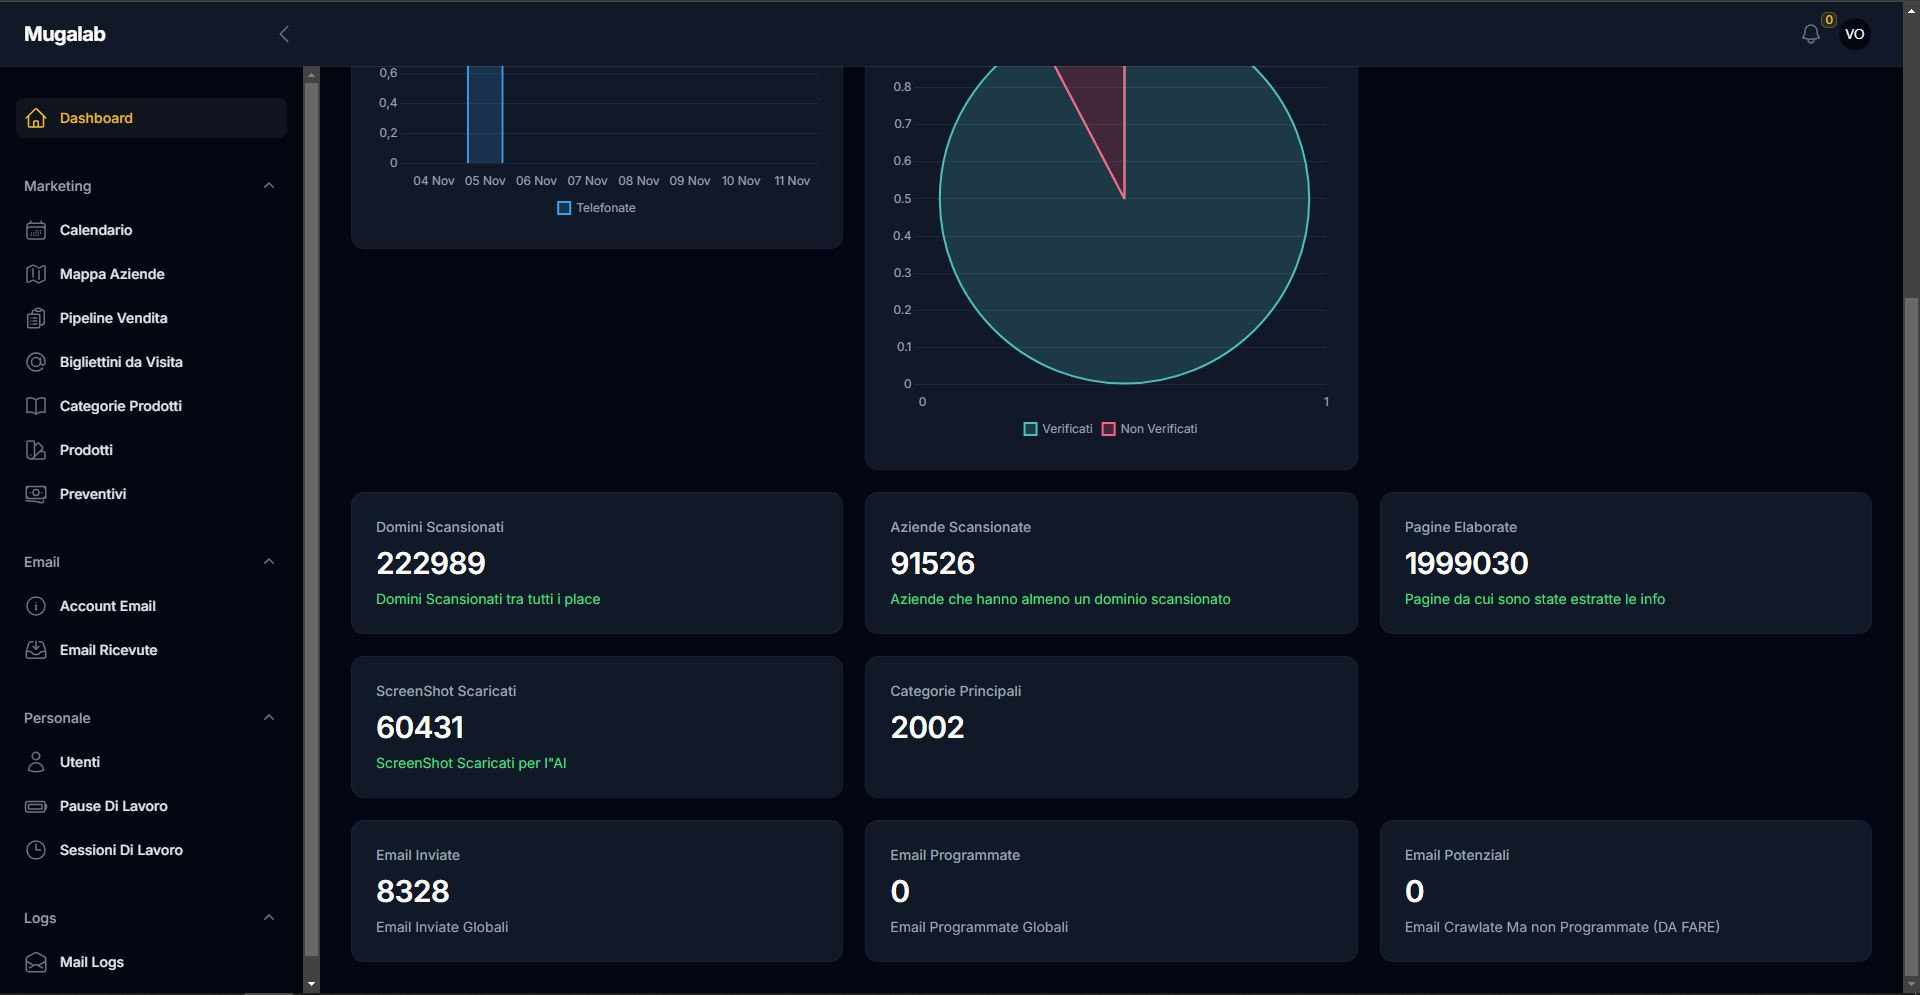
\includegraphics[width=0.8\columnwidth]{progetto/Home_page.png} 
        \caption{Home page di SalesCRM}
        \label{fig:salesCRM-home}
      \end{figure}

    \item Il modulo contenente il calendario (Fig.~\ref{fig:salesCRM-calendario}) è utile per pianificare appuntamenti e visite.
    
    \begin{figure}[!h] 
        \centering 
        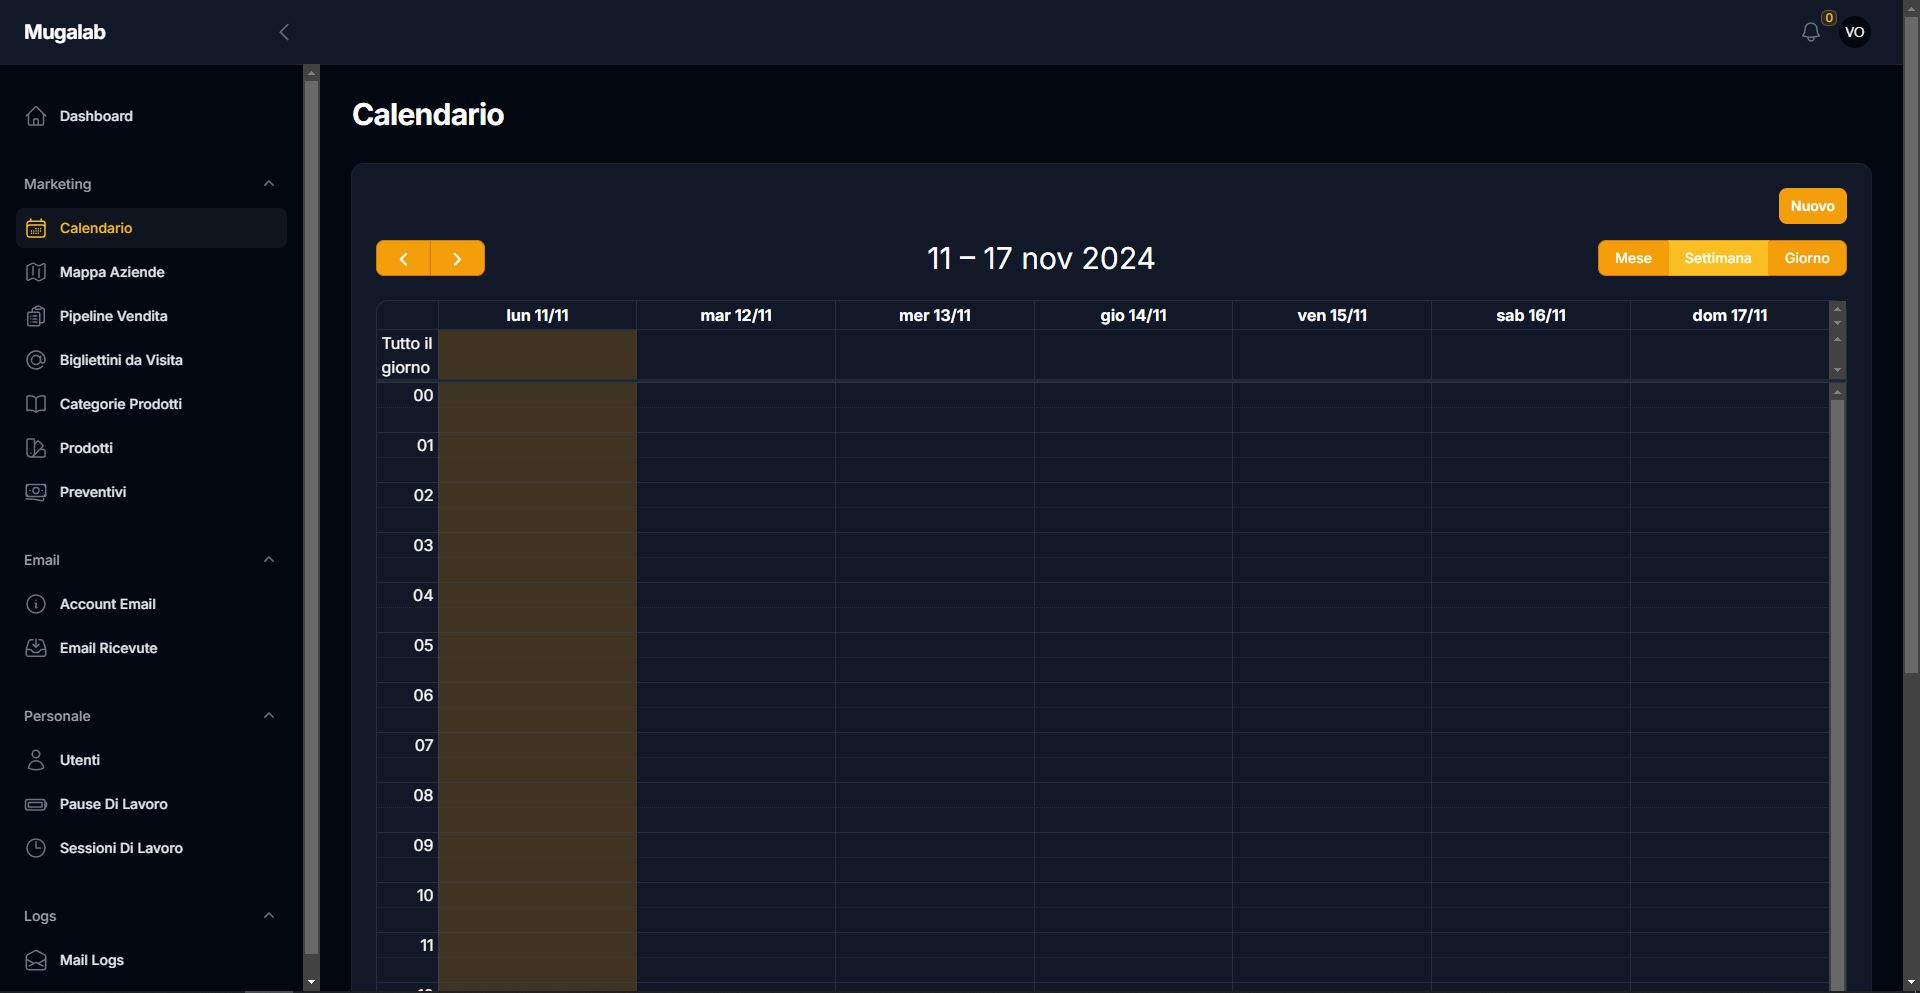
\includegraphics[width=0.8\columnwidth]{progetto/Calendario.png} 
        \caption{Calendario contenuto all'interno di SalesCRM}
        \label{fig:salesCRM-calendario}
      \end{figure}

    \item La sezione della mappa (Fig.~\ref{fig:salesCRM-mappa}) viene sfruttato per conoscere il posizionamento dei clienti e organizzare incontri locali.
    
    \begin{figure}[!h] 
        \centering 
        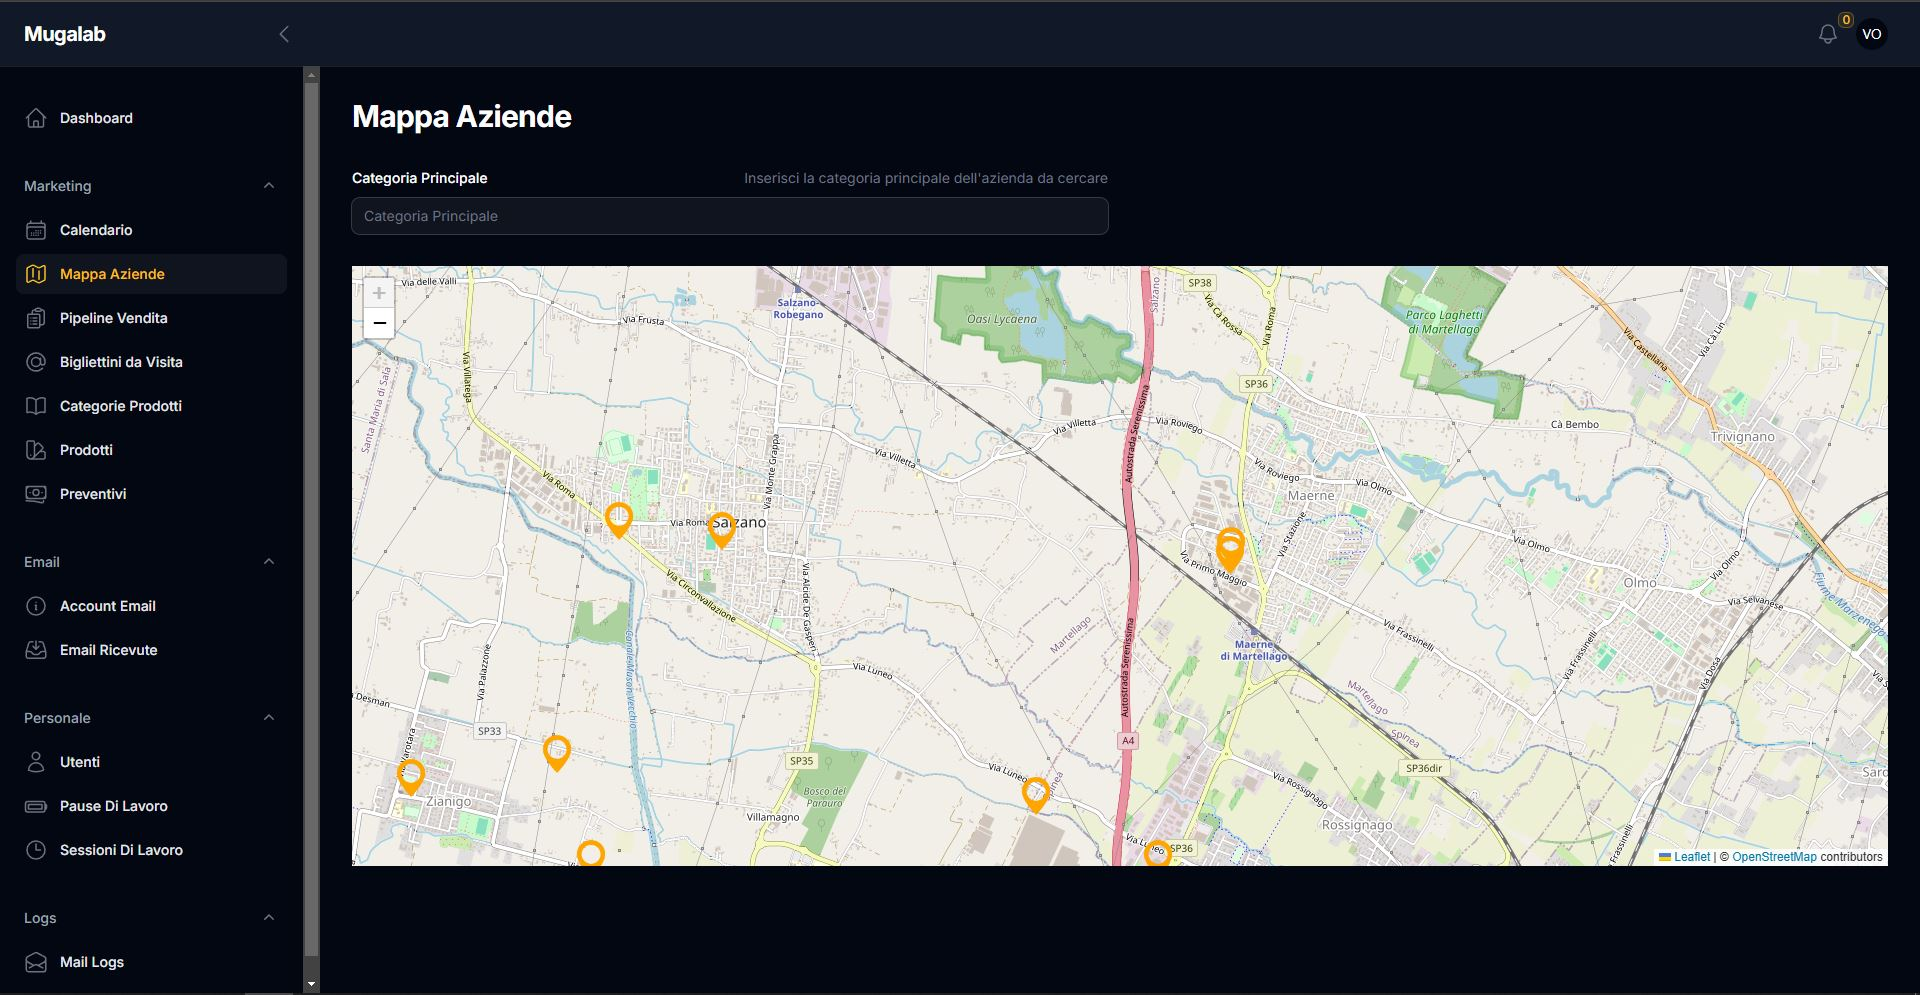
\includegraphics[width=0.8\columnwidth]{progetto/Mappa.png} 
        \caption{Mappa contenuta all'interno di SalesCRM}
        \label{fig:salesCRM-mappa}
      \end{figure}
    
\end{itemize}

\newpage

\subsection{Integrazione}
\begin{itemize}
    \item Raccolta di dati: l'applicativo ha una funzionalità di web-scraping che raccoglie i link dei siti web di tutti i potenziali clienti, il compito del tirocinante è quello di creare un workflow automatico che si integri con il web-scraper per acquisire screenshot delle varie pagine del sito web. 
    \item Clusterizzazione: la fase successiva alla raccolta dei dati consiste nello sviluppo di una IA addestrata in maniera non supervisionata che sia in grado di suddividere le varie immagini in clusters, differenziati in base alle caratteristiche riconosciute in ogni sito. 
    \item IA classificativa: in seguito alla raccolta di un dataset di dimensioni congrue si procede alla suddivisione manuale degli screenshot precedentemente clusterizzati su una base qualitativa (siti migliorabili e siti ottimi); questo processo viene svolto con l'ottica dell'addestramento di una IA classificativa.
    L'IA addestrata in maniera supervisionata ha l'obiettivo di affidare un punteggio in valori centesimali a ogni sito. 
    \item Invio di e-mail automatizzato: l'automazione della posta elettronica procede con l'invio di e-mail personalizzate ai proprietari dei siti web che hanno ricevuto una valutazione scarsa, per offrire loro un servizio di miglioramento.
\end{itemize}

\section{Analisi e gestione dei rischi}
Durante l'analisi del progetto lo stagista ha individuato alcuni rischi in cui potrà incorrere.
Nella lista seguente sono elencati i rischi e le soluzioni ideate.\\

\begin{risk}{Rimodulazione dell'attività}
    \riskdescription{dopo un mese dall’inizio dello stage lo studente è stato riposizionato sul progetto attuale scartando il progetto precedente e trovandosi dunque con meno settimane a disposizione per la produzione}
    \risksolution{ridimensionamento delle attività e richieste di supporto più frequenti}
    \label{risk: tempistiche ristrette} 
\end{risk}

\begin{risk}{Approccio sperimentale}
    \riskdescription{il progetto prevede dei contributi originali e sperimentali per cui non sono disponibili soluzioni già pronte}
    \risksolution{auto apprendimento tramite tutorial on-line e richiesta di coinvolgimento di colleghi più esperti nell'ambito}
    \label{risk:conoscenze scarse} 
\end{risk}

\begin{risk}{Costo dell'Addestramento}
    \riskdescription{l'addestramento dell'intelligenza artificiale richiede l'utilizzo di potenti GPU di cui spesso l'hardware a disposizione è sprovvisto}
    \risksolution{utilizzo del server aziendale per l’addestramento su CPU, ottenendo un compromesso tra costi e tempo di addestramento}
    \label{risk:hardware} 
\end{risk}

\begin{risk}{Quantità di dati di training insufficiente}
    \riskdescription{l'IA necessita una grande quantità di dati in input per effettuare un training efficace}
    \risksolution{aumento manuale del dataset e ricerca di dataset già pronti on-line}
    \label{risk:hardware} 
\end{risk}

%AGGIUNGERE ALTRI RISCHI versioni dipendenti da altre

\newpage

\begin{risk}{Risultati della clusterizzazione non soddisfacenti}
    \riskdescription{il clustering potrebbe risultare non conforme alle aspettative}
    \risksolution{valutare la quantità di cluster da creare e sperimentare con altri metodi di clustering}
    \label{risk:hardware} 
\end{risk}


\begin{risk}{Overfitting del modello}
    \riskdescription{il modello IA fornisce valutazioni accurate solo per le immagini utilizzate durante il training}
    \risksolution{sperimentare con metodi per la risoluzione dell'overfit (dropout, cross-validation, ecc...)}
    \label{risk:hardware} 
\end{risk}

\begin{risk}{Dipendenze delle librerie}
    \riskdescription{il progetto utilizza molte tecnologie e librerie differenti, è probabile che si presentino delle incompatibilità}
    \risksolution{utilizzo del minor numero possibile di librerie e verifica delle compatibilità prima dell'inizio della scrittura del codice}
    \label{risk:hardware} 
\end{risk}

\section{Obiettivi}
Gli obiettivi hanno lo scopo di delineare il percorso che lo studente deve affrontare per portare a termine il progetto nella maniera desiderata dall'azienda.
Sono suddivisibili in:
\begin{itemize}
    \item \textbf{O}: obbligatori
    \item \textbf{D}: desiderabili
    \item \textbf{F}: facoltativi
\end{itemize}

\begin{table}[h!]
    \centering
    \begin{tabularx}{0.8\textwidth}{|c|X|}
    \hline
    \textbf{Codice} & \textbf{Descrizione} \\
    \hline
    O01 & Implementare un sistema robusto per la cattura degli screenshot, assicurando l’integrazione con il database per l’archiviazione e l’analisi. \\
    \hline
    O02 & Garantire la creazione di una documentazione tecnica completa che supporti sia l’uso che la manutenzione  del sistema sviluppato. \\
    \hline
    O03 & Creazione di un IA in grado di suddividere in cluster i siti web. \\
    \hline
    O04 & Creazione di un IA classificativa in grado di assegnare un punteggio ai siti-web analizzati.\\
    \hline
    D01 & Aggiungere la valutazione creata dall'IA nel database utilizzato dal CRM.\\
    \hline
    D02 & Automatizzare l'invio di e-mail alle aziende che hanno ottenuto una valutazione scarsa.\\
    \hline
    F01 & Migliorare la raccolta dei dati delle aziende dal web\\
    \hline
    F02 & Aggiornare automaticamente la valutazione dei siti web\\
    \hline
    \end{tabularx}
    \caption{Tabella degli obiettivi}
    \end{table}

%AGGIUNGERE SE HO TROPPE POCHE PAGINE
%\section{Pianificazione}

